%I hate this template
\newpage
\subsection{NAT}
Network Address Translation (NAT) is a commonly used technique among small to mid-sized ISPs for conserving public IP addresses and managing internal networks. 
Although NAT is a standard practice, it introduces additional complexity into packet forwarding.
Specifically, NAT requires the router to maintain stateful information for each active connection. 
For every translated flow, the router must store the original and translated source IP addresses and ports, along with the destination address and protocol type. 
This information is necessary to correctly map incoming response packets back to the appropriate internal hosts.
Since NAT modifies headers -- such as the source IP addresses and source ports -- all affected checksums must be recalculated, which imposes further computational overhead.
The goal of this test is to evaluate how NAT impacts overall system performance.

For this purpose, source NAT is applied on top of the one-way forwarding scenario, meaning that the test setup is identical to the basic forwarding case, but with NAT translation enabled at the DUT. 
A /16 source IP address pool is used to emulate a large number of concurrent clients, while the DUT has a /24 pool of inside global IP addresses available for translation. 
This configuration serves as a stress test for the NAT implementation and its capacity to manage many concurrent state entries.
NAT was implemented using \textit{nftables} in Linux, and the \textit{nat\_plugin} in VPP.

A one-way traffic pattern is used to isolate the performance impact of NAT translations without interference from return traffic, 
as response packets would be subject to the same translation and state tracking processes, merely in the opposite direction.

%----------------------------------
%----------------------------------
%----------------------------------
\subsubsection{1 Gbps Test Results}

As the results in Table~\ref{tab:nat-1g} show, the introduction of NAT had a slight impact on all VPP configurations compared to plain one-way forwarding at 1~Gbit/s.  
All VPP configurations also exhibited a consistent packet loss of approximately 1.5\%.
Since this behavior is present across all test cases, it suggests that VPP may drop the first few packets of each flow until a NAT session table entry is established.  
The stateless UDP traffic generated by TRex provides very limited context for session tracking, which likely contributes to this issue.  
In real-world network traffic -- typically bidirectional and stateful -- this behavior would likely not occur or would be mitigated by application-layer retries.
Interestingly, Linux delivered all packets with low latency except in the 64-byte frame test.  
The slightly better results of Linux with NAT compared to plain forwarding may be explained by the presence of precomputed conntrack sessions, which can accelerate routing decisions in the kernel.

\begin{table}[h!]
\centering
\caption{Results of NAT 1~Gbit/s tests}
\begin{tabular}{|c|l|r|r|r|r|}
\hline
\textbf{} & \textbf{Config} & \textbf{Energy [Wh]} & \textbf{Pkt Loss [\%]} & \textbf{Avg Lat [$\mu$s]} & \textbf{Jitter [$\mu$s]} \\
\hline
\multirow{4}{*}{\rotatebox{90}{64B}} &
          VPP-1  & 5.67  & 1.56  & 19.10 & 11.65 \\
        & VPP-4  & 6.37  & 1.56  & 35.75 & 16.35 \\
        & VPP-10 & 7.98  & 1.56  & 31.60 & 15.20  \\
        & Linux  & 6.61  & 4.43  & 303.25 & 182.85 \\
\hline
\multirow{4}{*}{\rotatebox{90}{512B}} &
          VPP-1  & 5.76  &  1.53 & 12.25  & 12.25 \\
        & VPP-4  & 6.36  &  1.53 & 26.60  & 19.30 \\
        & VPP-10 & 7.90  &  1.53 & 25.60  & 18.25 \\
        & Linux  & 6.21  &  0.00 & 18.50  & 10.25 \\
\hline
\multirow{4}{*}{\rotatebox{90}{889B}} &
          VPP-1  & 5.74  & 1.50  & 10.30  & 7.45   \\
        & VPP-4  & 6.26  & 1.50  & 23.40  & 18.40  \\
        & VPP-10 & 7.81  & 1.51  & 23.80  & 20.10  \\
        & Linux  & 6.13  & 0.00  & 12.30  & 11.30  \\
\hline
\multirow{4}{*}{\rotatebox{90}{1280B}} &
          VPP-1  & 5.73  & 1.48  & 7.70  &  7.30 \\
        & VPP-4  & 6.35  & 1.48  & 18.45 & 15.45 \\
        & VPP-10 & 7.75  & 1.48  & 19.10 & 16.45    \\
        & Linux  & 6.07  & 0.00  & 11.40  & 1.30   \\
\hline
\multirow{4}{*}{\rotatebox{90}{1518B}} &
          VPP-1  & 5.68  & 1.47  & 7.30  & 5.55  \\
        & VPP-4  & 6.35  & 1.47  & 17.55 & 16.50  \\
        & VPP-10 & 7.86  & 1.47  & 17.5  & 15.85 \\
        & Linux  & 6.05  & 0.00  & 10.55 & 6.60  \\
\hline
\end{tabular}
\label{tab:nat-1g}
\end{table}

The energy efficiency graph shown in Fig.~\ref{fig:nat-1g} demonstrates results similar to those observed in plain one-way 1\,Gbit/s forwarding.

\begin{figure}[!htbp]
    \centering
    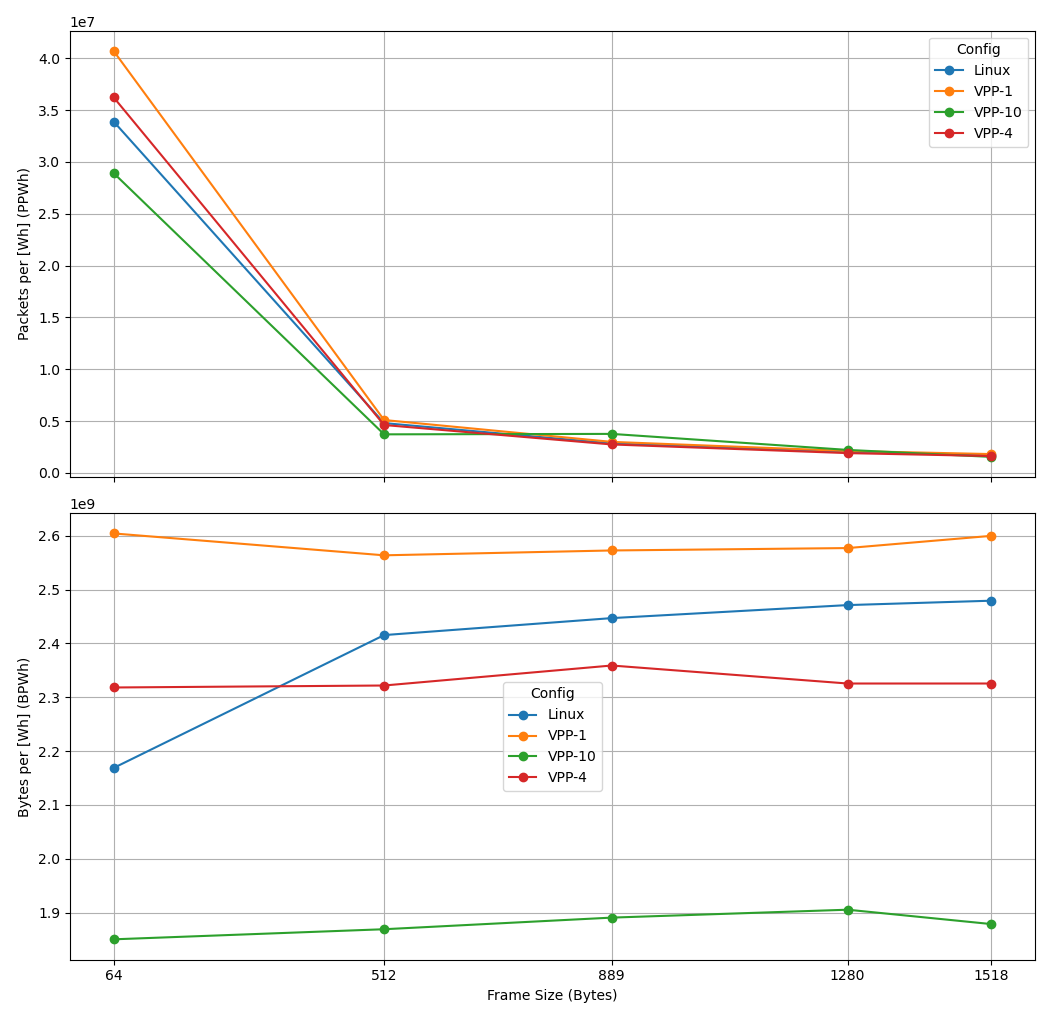
\includegraphics[width=\linewidth]{images/consumption-nat-1g.png}
    \caption{Energy efficiency per delivered data in NAT 1\,Gbit/s}
    \label{fig:nat-1g}
\end{figure}

%----------------------------------
%----------------------------------
%----------------------------------
\subsubsection{10 Gbps Test Results}

In this high-traffic scenario, the results presented in Table~\ref{tab:nat-10g} show that the increased packet rate had a noticeable impact on the Linux stack -- 
particularly in tests with smaller frame sizes -- resulting in significantly worse performance compared to plain 10~Gbit/s one-way forwarding. 
This highlights the considerable computational overhead introduced by NAT when combined with packet forwarding, especially at high packet-per-second rates.
VPP also exhibited some performance degradation in the 64-byte frame test compared to forwarding-only test. 
However, in all other cases, VPP maintained performance close to the plain forwarding baseline, with only minor differences. 
These results clearly demonstrate VPP’s superior packet processing efficiency over the Linux network stack under heavy NAT workloads.

\begin{table}[h!]
\centering
\caption{Results of NAT 10~Gbit/s tests}
\begin{tabular}{|c|l|r|r|r|r|}
\hline
\textbf{} & \textbf{Config} & \textbf{Energy [Wh]} & \textbf{Pkt Loss [\%]} & \textbf{Avg Lat [$\mu$s]} & \textbf{Jitter [$\mu$s]} \\
\hline
\multirow{4}{*}{\rotatebox{90}{64B}} &
          VPP-1  & 5.75  & 75.12 & 259.15 & 11.95 \\
        & VPP-4  & 6.17  & 51.98 & 735.00 & 55.20 \\
        & VPP-10 & 7.95  & 5.86  & 676.15 & 76.15 \\
        & Linux  & 7.25  & 84.03 & 10314.40 & 1683.40 \\
\hline
\multirow{4}{*}{\rotatebox{90}{512B}} &
          VPP-1  & 5.56  & 1.56  & 31.15 & 16.90 \\
        & VPP-4  & 6.20  & 1.56  & 40.10 & 17.45 \\
        & VPP-10 & 7.76  & 1.56  & 32.40 & 17.65 \\
        & Linux  & 6.87  & 9.02  & 255.10 & 177.45  \\
\hline
\multirow{4}{*}{\rotatebox{90}{889B}} &
          VPP-1  & 5.57  & 1.56  & 29.80 & 18.55 \\
        & VPP-4  & 6.28  & 1.56  & 34.45 & 21.60 \\
        & VPP-10 & 7.78  & 1.56  & 29.45 & 17.00 \\
        & Linux  & 6.63  & 0.00  & 166.20 & 129.60 \\
\hline
\multirow{4}{*}{\rotatebox{90}{1280B}} &
          VPP-1  & 5.66  & 1.55  & 26.65 & 18.10 \\
        & VPP-4  & 6.26  & 1.55  & 31.50 & 19.50 \\
        & VPP-10 & 7.79  & 1.56  & 28.55 & 17.20 \\
        & Linux  & 6.49  & 0.00  & 101.20 & 93.40  \\
\hline
\multirow{4}{*}{\rotatebox{90}{1518B}} &
          VPP-1  & 5.64  & 1.55  &  26.10 & 18.20  \\
        & VPP-4  & 6.21  & 1.55  &  30.15 & 19.35  \\
        & VPP-10 & 7.88  & 1.55  &  26.55 & 18.60  \\
        & Linux  & 6.45  & 0.00  &  67.25 & 61.60  \\
\hline
\end{tabular}
\label{tab:nat-10g}
\end{table}

The energy efficiency graph in Fig.~\ref{fig:nat-10g} shows results that closely mirror those observed in the plain one-way 10\,Gbps forwarding test. 
The only notable deviation is the reduced performance of the VPP-4 configuration in the 64-byte frame scenario.

\begin{figure}[!htbp]
    \centering
    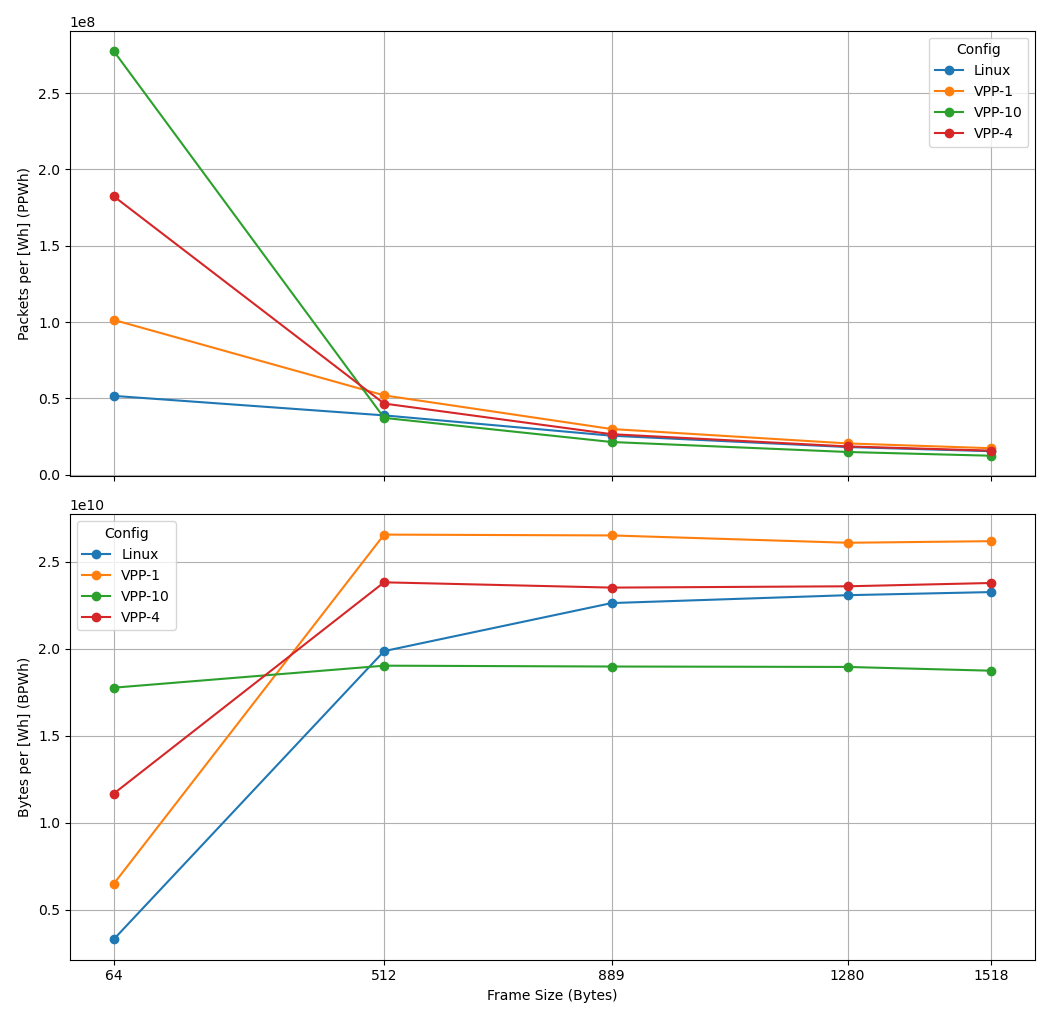
\includegraphics[width=\linewidth]{images/consumption-nat-10g.png}
    \caption{Energy efficiency per delivered data in NAT 10\,Gbit/s}
    \label{fig:nat-10g}
\end{figure}

%----------------------------------
%----------------------------------
%----------------------------------
\subsubsection{25 Gbps Test Results}

As shown in Table~\ref{tab:nat-25g}, even the VPP-10 configuration dropped more than half of all packets in the 64-byte frame scenario. 
All VPP configurations experienced a noticeable spike in packet loss rates, particularly in the 64-byte frame test. 
The results in this test are more comparable to the 40Gbit/s basic forwarding scenario than to the 25Gbit/s one.
In the remaining frame size tests, all VPP latency metrics approximately doubled compared to basic 25~Gbit/s forwarding. The Linux configuration, once again, struggled with high latency and severe packet loss.
Overall, these findings further demonstrate VPP’s capability to handle high-throughput traffic -- although NAT processing introduces a significant computational burden. 

\begin{table}[h!]
\centering
\caption{Results of NAT 25~Gbit/s tests}
\begin{tabular}{|c|l|r|r|r|r|}
\hline
\textbf{} & \textbf{Config} & \textbf{Energy [Wh]} & \textbf{Pkt Loss [\%]} & \textbf{Avg Lat [$\mu$s]} & \textbf{Jitter [$\mu$s]} \\
\hline
\multirow{4}{*}{\rotatebox{90}{64B}} &
          VPP-1  & 5.73  & 90.19 & 459.65 & 17.80 \\
        & VPP-4  & 6.39  & 80.63 & 836.1  & 58.95 \\
        & VPP-10 & 7.95  & 59.86 & 851.35 & 57.60 \\
        & Linux  & 7.26  & 93.62 & 8398.85 & 1636.1 \\
\hline
\multirow{4}{*}{\rotatebox{90}{512B}} &
          VPP-1  & 5.70  & 23.82 & 256.05 & 23.55 \\
        & VPP-4  & 6.50  & 1.56  & 71.55 & 23.05  \\
        & VPP-10 & 7.95  & 1.56  & 40.05 & 15.85  \\
        & Linux  & 7.30  & 51.35 & 4566.95 & 408.6 \\
\hline
\multirow{4}{*}{\rotatebox{90}{889B}} &
          VPP-1  & 5.63  & 1.57  & 44.10 & 30.15 \\
        & VPP-4  & 6.61  & 1.56  & 47.45 & 21.40 \\
        & VPP-10 & 7.91  & 1.56  & 35.70 & 21.30 \\
        & Linux  & 7.02  & 28.91 & 6797.05 & 403.45 \\
\hline
\multirow{4}{*}{\rotatebox{90}{1280B}} &
          VPP-1  & 5.70  & 1.56  & 35.10 & 15.95 \\
        & VPP-4  & 6.63  & 1.56  & 43.05 & 21.60 \\
        & VPP-10 & 7.95  & 1.56  & 36.70 & 18.20 \\
        & Linux  & 6.92  & 12.54 & 262.25 & 204.50  \\
\hline
\multirow{4}{*}{\rotatebox{90}{1518B}} &
          VPP-1  & 5.81 & 1.56  & 31.20 & 14.40 \\
        & VPP-4  & 6.63 & 1.56  & 40.65 & 22.50 \\
        & VPP-10 & 8.03 & 1.56  & 34.40 & 18.45 \\
        & Linux  & 6.82 & 2.25  & 282.15 & 175.4  \\
\hline
\end{tabular}
\label{tab:nat-25g}
\end{table}

The energy efficiency graph in Fig.~\ref{fig:nat-25g} shows results broadly similar to those observed in the plain one-way 25,Gbps forwarding scenario. 
However, the Linux configuration performed slightly worse in terms of BPWh and PPWh, falling behind the VPP-10 configuration in the 889-byte frame scenario.

\begin{figure}[!htbp]
    \centering
    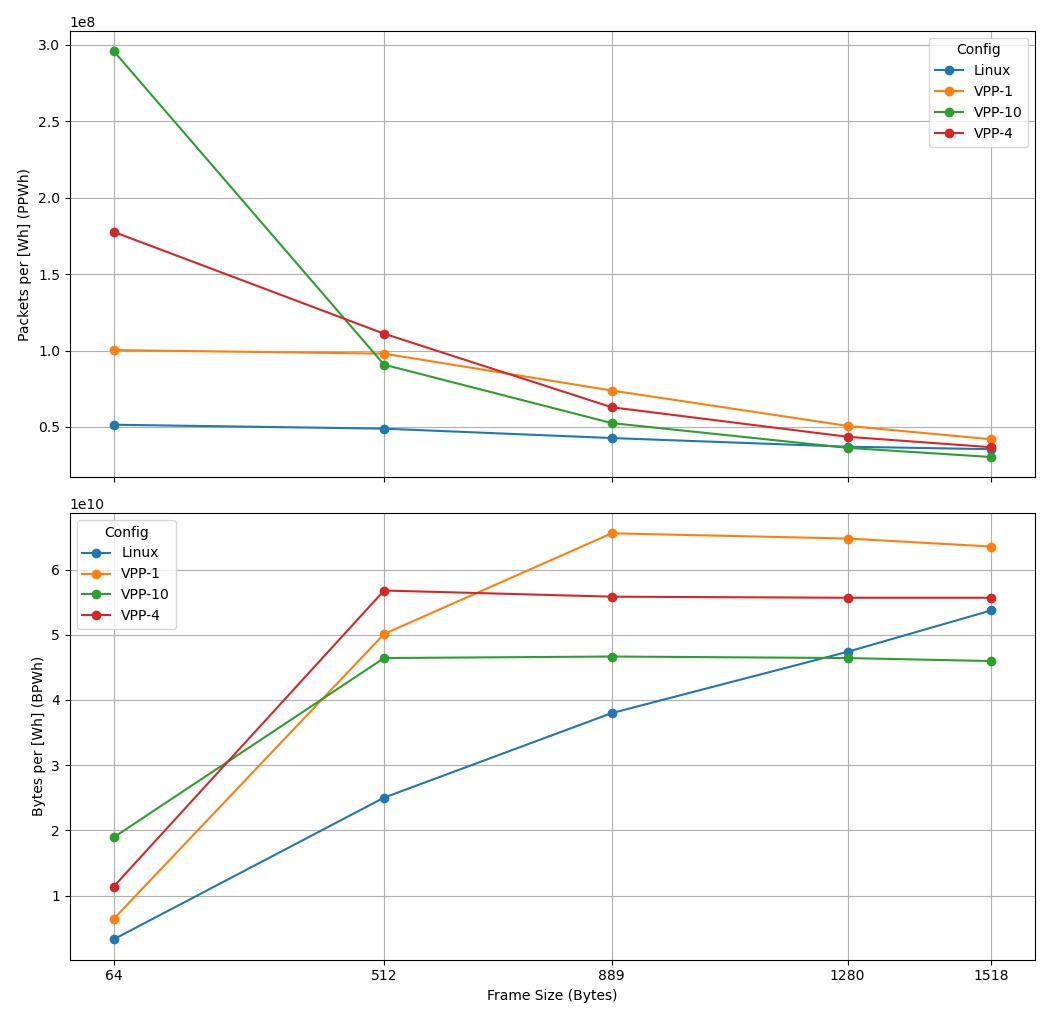
\includegraphics[width=\linewidth]{images/consumption-nat-25g.png}
    \caption{Energy efficiency per delivered data in NAT 25\,Gbit/s}
    \label{fig:nat-25g}
\end{figure}





%----------------------------------
%----------------------------------
%----------------------------------
\subsubsection{40 Gbps Test Results}

The results of the most extreme NAT test presented in Table \ref{tab:nat-40g} continue the trend observed in the previous test.
In scenarios where VPP handled almost the full processing of traffic, the average latency in some cases nearly doubled compared to pure forwarding in the 40 Gbit/s test.

\begin{table}[h!]
\centering
\caption{Results of NAT 40~Gbit/s tests}
\begin{tabular}{|c|l|r|r|r|r|}
\hline
\textbf{} & \textbf{Config} & \textbf{Energy [Wh]} & \textbf{Pkt Loss [\%]} & \textbf{Avg Lat [$\mu$s]} & \textbf{Jitter [$\mu$s]} \\
\hline
\multirow{4}{*}{\rotatebox{90}{64B}} &
          VPP-1  & 5.78  & 93.89 & 447.95 & 16.60 \\
        & VPP-4  & 6.41  & 87.59 & 830.80 & 44.80 \\
        & VPP-10 & 7.98  & 74.47 & 860.45 & 55.85 \\
        & Linux  & 7.21  & 95.71 & 3507.75 & 456.25  \\
\hline
\multirow{4}{*}{\rotatebox{90}{512B}} &
          VPP-1  & 5.79  & 52.02 & 264.75 & 18.45  \\
        & VPP-4  & 6.61  & 17.80 & 793.65 & 64.10  \\
        & VPP-10 & 8.00  & 1.56  & 49.75  & 17.15  \\
        & Linux  & 7.32  & 63.20 & 3017.60 & 287.65  \\
\hline
\multirow{4}{*}{\rotatebox{90}{889B}} &
          VPP-1  &  5.82 & 21.93 & 324.95 & 33.50 \\
        & VPP-4  &  6.62 & 1.56  & 65.25  & 22.60 \\
        & VPP-10 &  8.05 & 1.56  & 44.10  & 17.90  \\
        & Linux  &  7.43 & 39.44 & 2838.95 & 127.05 \\
\hline
\multirow{4}{*}{\rotatebox{90}{1280B}} &
          VPP-1  & 5.85  & 1.61  & 71.20 & 24.95 \\
        & VPP-4  & 6.59  & 1.56  & 51.60 & 21.25 \\
        & VPP-10 & 7.98  & 1.56  & 41.60 & 19.95 \\
        & Linux  & 7.15  & 35.39 & 5840.10 & 313.60  \\
\hline
\multirow{4}{*}{\rotatebox{90}{1518B}} &
          VPP-1  & 5.86  & 1.57  & 48.65 & 26.90 \\
        & VPP-4  & 6.59  & 1.56  & 47.80 & 20.60 \\
        & VPP-10 & 8.10  & 1.56  & 39.00 & 19.45 \\
        & Linux  & 7.09  & 26.47 & 7408.65 &  350.9  \\
\hline
\end{tabular}
\label{tab:nat-40g}
\end{table}

As shown in the energy efficiency graph in Fig.~\ref{fig:nat-40g}, Linux was the least energy-efficient option, performing worse than any of the VPP configurations. 
Even VPP-1 showed slightly lower efficiency compared to the other VPP setups, and in the 889-byte frame scenario, its performance dropped below that of VPP-4.

\begin{figure}[!htbp]
    \centering
    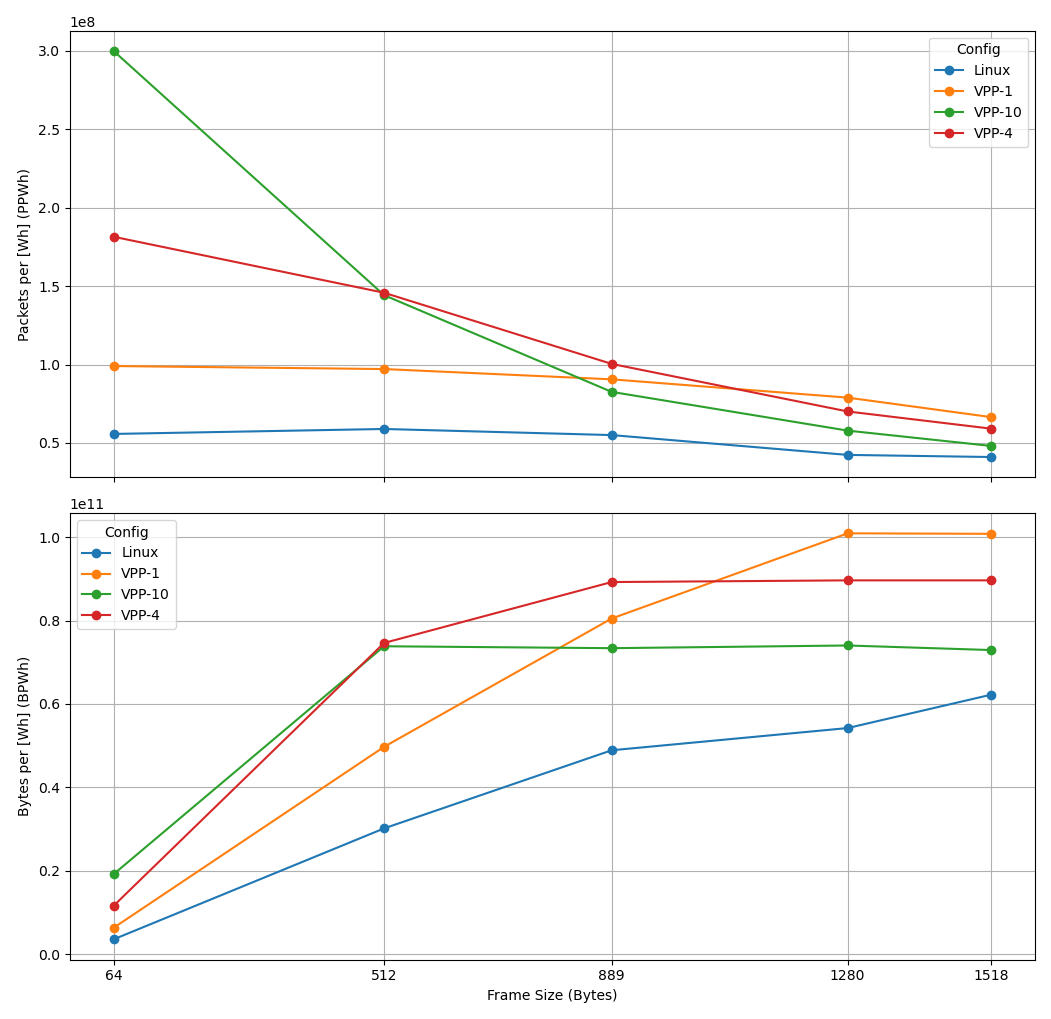
\includegraphics[width=\linewidth]{images/consumption-nat-40g.png}
    \caption{Energy efficiency per delivered data in NAT 40\,Gbit/s}
    \label{fig:nat-40g}
\end{figure}

